%%%%%%%%%%%%%%%%%%%%%%%%%%%%%%%%%%%%%%%%%
% University/School Laboratory Report
% LaTeX Template
% Version 3.1 (25/3/14)
%
% This template has been downloaded from:
% http://www.LaTeXTemplates.com
%
% Original author:
% Linux and Unix Users Group at Virginia Tech Wiki 
% (https://vtluug.org/wiki/Example_LaTeX_chem_lab_report)
%
% License:
% CC BY-NC-SA 3.0 (http://creativecommons.org/licenses/by-nc-sa/3.0/)
%
%%%%%%%%%%%%%%%%%%%%%%%%%%%%%%%%%%%%%%%%%

%----------------------------------------------------------------------------------------
%	PACKAGES AND DOCUMENT CONFIGURATIONS
%----------------------------------------------------------------------------------------

\documentclass{article}

\usepackage[version=3]{mhchem} % Package for chemical equation typesetting
\usepackage{siunitx} % Provides the \SI{}{} and \si{} command for typesetting SI units
\usepackage{graphicx} % Required for the inclusion of images
\usepackage{natbib} % Required to change bibliography style to APA
\usepackage{amsmath} % Required for some math elements 
\usepackage{caption}
\usepackage{subcaption}
\usepackage{listings}
\usepackage{color}
 
\definecolor{codegreen}{rgb}{0,0.6,0}
\definecolor{codegray}{rgb}{0.5,0.5,0.5}
\definecolor{codepurple}{rgb}{0.58,0,0.82}
\definecolor{backcolour}{rgb}{0.95,0.95,0.92}
 
\lstdefinestyle{mystyle}{
    backgroundcolor=\color{backcolour},   
    commentstyle=\color{codegreen},
    keywordstyle=\color{codepurple},
    numberstyle=\tiny\color{codegray},
    stringstyle=\color{codepurple},
    basicstyle=\footnotesize,
    emph={
      cudaMalloc, cudaFree,
      __global__, __shared__, __device__, __host__,
      __syncthreads,
    },
    breakatwhitespace=false,         
    breaklines=true,                 
    captionpos=b,                    
    keepspaces=true,                 
    numbers=left,                    
    numbersep=5pt,                  
    showspaces=false,                
    showstringspaces=false,
    showtabs=false,                  
    tabsize=2
}
\lstset{style=mystyle}

\setlength\parindent{0pt} % Removes all indentation from paragraphs

\renewcommand{\labelenumi}{\alph{enumi}.} % Make numbering in the enumerate environment by letter rather than number (e.g. section 6)

\newcommand\tab[1][0.5cm]{\hspace*{#1}}

%\usepackage{times} % Uncomment to use the Times New Roman font

%----------------------------------------------------------------------------------------
%	DOCUMENT INFORMATION
%----------------------------------------------------------------------------------------

\title{COMP 429/529: Project 3} % Title

\author{
  Berkay \textsc{Barlas} \\54512
  \and
  Naim Berk \textsc{Tumer} \\53847
}
\date{\today} % Date for the report

\begin{document}

\maketitle % Insert the title, author and date

\begin{center}
\begin{tabular}{l r}
Date Performed: & March 17, 2019 \\ % Date the experiment was performed
Instructor: & Didem Unat % Instructor/supervisor
\end{tabular}
\end{center}

% If you wish to include an abstract, uncomment the lines below
% \begin{abstract}
% Abstract text
% \end{abstract}

%----------------------------------------------------------------------------------------
%	SECTION 1
%----------------------------------------------------------------------------------------

\tab In this assignment we implemented CUDA versions
on top of given serial version for Cardiac Electrophysiology Simulation and conducted experiments. 
\\ \tab  To compile all the necessary files run \textbf{make}
\newline
In this assignment we have completed
\begin{itemize}
    \item Version 1: A naive that uses global (device) memory
    \item Version 2: All kernels fused into one kernel
    \item Version 3: Temporary variable references for R and E arrays 
    \item Version 4: Optimized for CUDA using shared on-chip memory with 2D blocks 
\end{itemize}

\section{Implementation}
\textbf{CUDA Implementations}

\subsection{Version 1}
\tab In this version, we parallelized the simulator using single GPU with a naive implementation that makes all the references to global (device) memory. 
\\ We created 3 different kernels for ode and pde and ghost cells.

\begin{lstlisting}[language=C++]
__global__ void ghosts(const int n, const int m, double *E_prev) {
    int j = threadIdx.x + 1;

    E_prev[j * (n+2)] = E_prev[j * (n+2) + 2];
    E_prev[j * (n+2) + (n + 1)] = E_prev[j * (n + 2) + (n - 1)];

    E_prev[j] = E_prev[2 * (n + 2) + j];
    E_prev[(m + 1) * (n + 2) + j] = E_prev[(m - 1) * (n + 2) + j];
}
\end{lstlisting}

\begin{lstlisting}[language=C++]
__global__ void ode(const double a, const double kk, const double dt, const int n, const int m, double *E, double *R,
                    const double epsilon,
                    const double M1, const double M2, const double b) {
    /*
     * Solve the ODE, advancing excitation and recovery to the
     *     next timtestep
       */
    int i = threadIdx.x + 1;
    int j = blockIdx.x + 1;
    int index = j * (n + 2) + i;

    E[index] = E[index] - dt * (kk * E[index] * (E[index] - a) * (E[index] - 1) + E[index] * R[index]);
    R[index] = R[index] + dt * (epsilon + M1 * R[index] / (E[index] + M2)) * (-R[index] - kk * E[index] * (E[index] - b - 1));
}
\end{lstlisting}

\begin{lstlisting}[language=C]
__global__ void pde(const int n, const int m, double *E, double *E_prev, const double alpha) {
	int i = threadIdx.x + 1;
	int j = blockIdx.x + 1;
	int index = j * (n + 2) + i;
	
    E[index] = E_prev[index] + alpha *
                               (E_prev[index + 1] + E_prev[index - 1] - 4 * E_prev[index] + E_prev[index + m + 2] +
                                E_prev[index - (m + 2)]);
}
\end{lstlisting}


\subsection{Version 2}
\tab In this version, we fused all the kernels into one kernel by can fusing the ODE and PDE loops into a single loop.

\begin{lstlisting}[language=C++]
__global__ void pde_ode(const double a, const double kk, const double dt, const int n, const int m, double *E, double *E_prev, double *R, 
    const double epsilon, const double M1, const double M2, const double b, const double alpha) {
    
    int i = threadIdx.x + 1;
    int j = blockIdx.x + 1;
    int index = j * (n + 2) + i;
     
    E[index] = E_prev[index] + alpha * (E_prev[index + 1] + E_prev[index - 1] - 4 * E_prev[index] + E_prev[index + m + 2] + E_prev[index - (m + 2)]);
    E[index] = E[index] - dt * (kk * E[index] * (E[index] - a) * (E[index] - 1) + E[index] * R[index]);
    R[index] = R[index] + dt * (epsilon + M1 * R[index] / (E[index] + M2)) * (-R[index] - kk * E[index] * (E[index] - b - 1));
 }
\end{lstlisting}

\subsection{Version 3}
\tab In this version, we used temporary variables to eliminate global memory references for R and E arrays in the ODEs.

\begin{lstlisting}[language=C++]
__global__ void pde_ode(const double a, const double kk, const double dt, const int n, const int m, double *E, double *E_prev, double *R, 
  const double epsilon, const double M1, const double M2, const double b, const double alpha) {
  
  int i = threadIdx.x + 1;
  int j = blockIdx.x + 1;
  int index = j * (n + 2) + i;

  double temp_E = E[index]; 
  double temp_R = R[index];
   
  temp_E = E_prev[index] + alpha * (E_prev[index + 1] + E_prev[index - 1] - 4 * E_prev[index] + E_prev[index + m + 2] + E_prev[index - (m + 2)]);
  temp_E = temp_E - dt * (kk * temp_E * (temp_E - a) * (temp_E - 1) + temp_E * temp_R);
  temp_R = temp_R + dt * (epsilon + M1 * temp_R / (temp_E + M2)) * (-temp_R - kk * temp_E * (temp_E - b - 1));

  E[index] = temp_E;
  R[index] = temp_R;
}
\end{lstlisting}

\newpage

\subsection{Version 4}
\tab In this version, we optimised our CUDA implementation by using shared on-chip memory on the GPU by bringing a 2D block into shared memory and sharing it with multiple threads in the same thread block.

\begin{lstlisting}[language=C++]
__global__ void pde_ode(const double a, const double kk, const double dt, const int n, const int m, double *E, double *E_prev, double *R, const double epsilon, const double M1, const double M2, const double b, const double alpha) {

  int tx = threadIdx.x, ty = threadIdx.y;
  int bx = blockIdx.x, by = blockIdx.y;
    
  __shared__ double block_E_prev[TILE_DIM + 2][TILE_DIM + 2];     
  if(tx == 0) {
      int index = (by * blockDim.y * (n + 2)) + (bx * blockDim.x) + ((ty + 1) * (n + 2));
      for (int j = 0; j < blockDim.x + 2; j++) {
          block_E_prev[ty + 1][j] = E_prev[index + j];
      }
      if(ty == 0) {
          int index = (by * blockDim.y * (n + 2)) + (bx * blockDim.x);
  
          for (int j = 0; j < blockDim.x + 2; j++) {
              block_E_prev[0][j] = E_prev[index + j];
          }
      }
      if(ty == 1) {
          int index = (by * blockDim.y * (n + 2)) + (bx * blockDim.x) + ((blockDim.y + 1) * (n + 2));
          for (int j = 0; j < blockDim.x + 2; j++) {
              block_E_prev[blockDim.y + 1][j] = E_prev[index + j];
          }
      }
  }  
  int index = (by * blockDim.y * (n + 2)) + (bx * blockDim.x) + (n + 2) + 1 + (ty * (n + 2) + tx);
  
  __syncthreads();

  double temp_E = E[index]; 
  double temp_R = R[index];
   
  temp_E = block_E_prev[ty + 1][tx + 1] + alpha * (block_E_prev[ty + 1][tx + 2] + block_E_prev[ty + 1][tx] - 4 * block_E_prev[ty + 1][tx + 1] + block_E_prev[ty + 2][tx + 1] + block_E_prev[ty][tx + 1]);
  temp_E = temp_E - dt * (kk * temp_E * (temp_E - a) * (temp_E - 1) + temp_E * temp_R);
  temp_R = temp_R + dt * (epsilon + M1 * temp_R / (temp_E + M2)) * (-temp_R - kk * temp_E * (temp_E - b - 1));
  __syncthreads();
  E[index] = temp_E;
  R[index] = temp_R;
}
\end{lstlisting}


%----------------------------------------------------------------------------------------
%	SECTION Studies
%----------------------------------------------------------------------------------------
\newpage

\section{Performance Report}
\subsection{Performance Study without plotter}

\tab We conducted a performance study without the plotter is on. In our results version 2 performed better in terms of execution time and gflops rate. We observed that data transfer time does not affects the performance significantly as we only copy the data at begining and end of execution. 
\\ \tab Version 2 performed better because of the required number of operations are minimum while in other version additional operations are needed such as copying data to a local variable and to a shared variable.
\\ \tab Version 4 performed worse than other versions because bringing block to shared memory take a lot of time. Moreover we tried different block sizes and observed version with block size 16 is best. 
\\
\\
Device: GeForce GTX 1080 Ti
 \begin{description}
    \item[Serial]: \hfill
      \begin{description} 
        \item[Execution Time (sec)]: 570.656\hfill 
        \item[Gflops Rate ]: 5.96103\hfill 
      \end{description}  
    \item[Version 1]: \hfill
      \begin{description} 
        \item[Execution Time (sec)]: 21.3603\hfill 
        \item[Gflops Rate ]: 159.253\hfill 
      \end{description} 
    \item[Version 2]: \hfill
      \begin{description} 
        \item[Execution Time (sec)]: 17.9579\hfill 
        \item[Gflops Rate ]: 189.426 \hfill 
      \end{description} 
    \item[Version 3]: \hfill
      \begin{description} 
        \item[Execution Time (sec)]: 18.123\hfill 
        \item[Gflops Rate ]: 187.701\hfill 
      \end{description}
    \item[Version 4 with Block size 16]: \hfill
      \begin{description} 
        \item[Execution Time (sec)]: 24.9325\hfill 
        \item[Gflops Rate ]: 136.436\hfill 
      \end{description}  
\end{description}
\begin{figure}[!htb]
  \centering
  \begin{subfigure}{.45\textwidth}
      \centering
      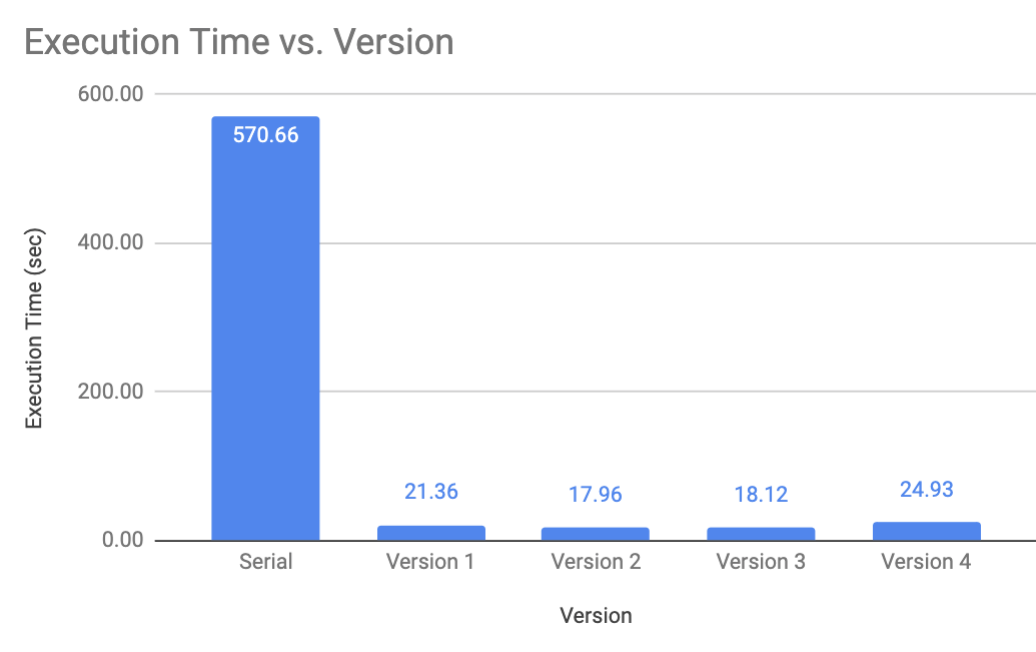
\includegraphics[width=1\linewidth]{./img/execution-version.png}
      \caption{Execution times of different versions}
  \end{subfigure} 
  \begin{subfigure}{.45\textwidth}
      \centering
      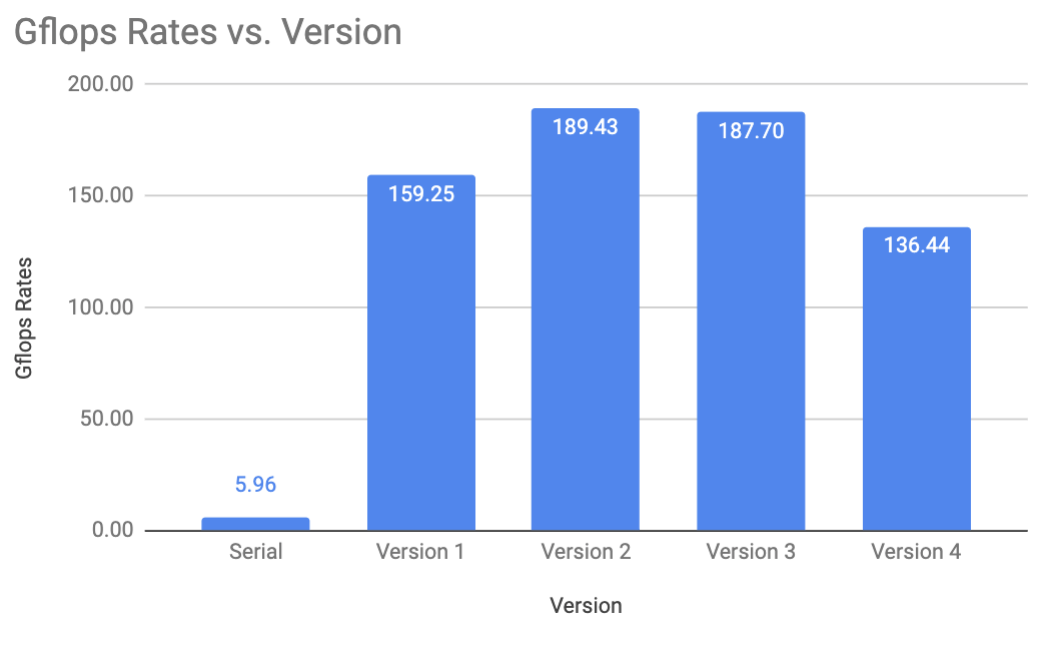
\includegraphics[width=1\linewidth]{./img/gflops-version.png}
      \caption{Gflops Rate of different versions}
  \end{subfigure}
  \caption{}
\end{figure}   

\newpage
%----------------------------------------------------------------------------------------
%	Comparison with Stream Benchmark
%----------------------------------------------------------------------------------------
\subsection{Comparison with Stream Benchmark}

\tab Stream Benchmark shows highest bandwidth rate that can be possible on the device. 
The highest Bandwidth rate we achieved is 216 GB/sec with Version 2 while the maximum device to device Bandwidth is 347 GB/sec. 

\begin{description}
  \item[Benchmark Results] \hfill
  \begin{description}
    \item [Host to Device Bandwidth (GB/sec): 11.688 ] \hfill
    \item [Device to Host Bandwidth (GB/sec): 12.723 ] \hfill
    \item [Device to Device Bandwidth (GB/sec): 347.221] \hfill
  \end{description}
  \item[Our Implementation]  \hfill
  \begin{description}
    \item[Serial Version Sustained Bandwidth (GB/sec):] 6.8126 \hfill 
    \item[Serial Version Sustained Bandwidth (GB/sec):] 6.8126 \hfill 
    \item[Version 1 Sustained Bandwidth (GB/sec):] 182.003 \hfill 
    \item[Version 2 Sustained Bandwidth (GB/sec):] 216.487\hfill 
    \item[Version 3 Sustained Bandwidth (GB/sec):] 214.515\hfill 
    \item[Version 4 with Block Size 64 Sustained Bandwidth (GB/sec):] 155.927 \hfill 
  \end{description}
\end{description}

\newpage

\subsection{Performance Results with Different Block Sizes}
\tab We conducted performance tests of version 4 with 4, 8, 16, 32 and 64 grid sizes. As the grid size increases the number of copy operations decreases. \\However, after grid size 16 we observed a decrease in performance. 
\\ \tab The implementation with block size 16 became fastest one amongs them. The block size with 64 didn't fit to the available thread number in GPU block, therefore, it didn't work.  
\begin{description}
  \item[Version 4 with Block size 4]: \hfill
    \begin{description} 
      \item[Execution Time (sec)]: 45.1086\hfill 
      \item[Gflops Rate]: 75.4113\hfill 
    \end{description}  
  \item[Version 4 with Block size 8]: \hfill
    \begin{description} 
      \item[Execution Time (sec)]: 27.3411\hfill 
      \item[Gflops Rate ]: 124.417\hfill 
    \end{description}
  \item[Version 4 with Block size 16]: \hfill
    \begin{description} 
      \item[Execution Time (sec)]: 24.9325\hfill 
      \item[Gflops Rate]: 136.436\hfill 
    \end{description}
  \item[Version 4 with Block size 32]: \hfill
    \begin{description} 
      \item[Execution Time (sec)]: 31.5012\hfill 
      \item[Gflops Rate]: 107.986\hfill 
    \end{description}      
\end{description}
\begin{figure}[!htb]
  \centering
  \begin{subfigure}{.45\textwidth}
      \centering
      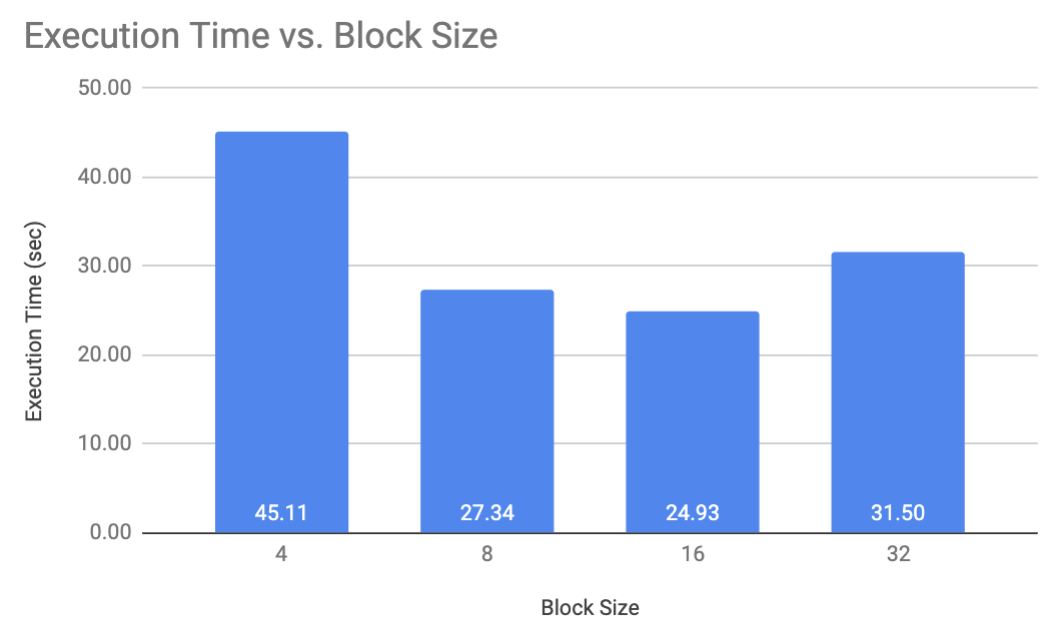
\includegraphics[width=1\linewidth]{./img/execution-block.png}
      \caption{Execution Times with respect to different block sizes}
  \end{subfigure} 
  \begin{subfigure}{.45\textwidth}
      \centering
      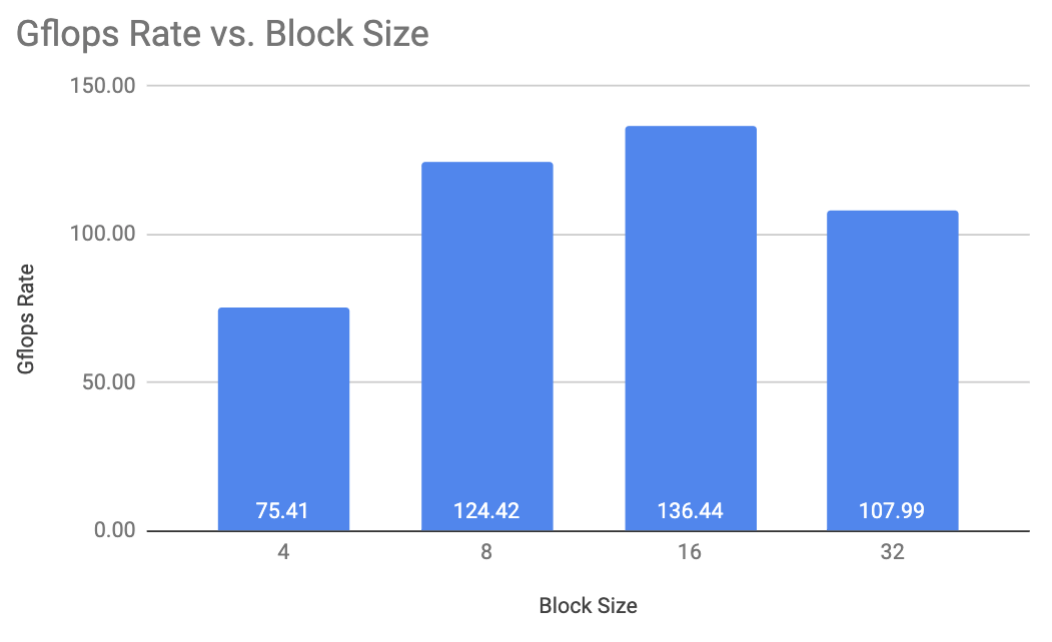
\includegraphics[width=1\linewidth]{./img/gflops-block.png}
      \caption{Gflops Rate results with different block sizes}

  \end{subfigure}
  \caption{}
\end{figure} 


\subsection{Serial vs CUDA}
\tab We observed a significant performance improvement with CUDA implementation. Our best CUDA implementation Version 2 is 33 times faster than serial version.
  \begin{description}
    \item[Serial Version]: \hfill
      \begin{description} 
        \item[Execution Time (sec)]: 570.656\hfill 
        \item[Gflops Rate ]: 5.96103\hfill 
      \end{description}  
    \item[CUDA]: Version 2\hfill
      \begin{description} 
        \item[Execution Time (sec)]: 17.9579\hfill 
        \item[Gflops Rate ]: 189.426 \hfill 
      \end{description} 
  \end{description}    

\subsection{MPI vs CUDA}
\tab Our CUDA implementation performed much better than our fastest MPI version with 32 thread and 8 x 4 geometry which was implemented in the second assignment. 
\\ \tab The difference between two implementations caused by commucation overhead such as updating the ghost cells in MPI version and the total number of threads used in calculations. While there are 32 threads in CPU, there are thousands of threads in GPU.
  \begin{description}
    \item[MPI Version 32 Thread 8 x 4]: \hfill
      \begin{description} 
        \item[Execution Time (sec)]: 448.854 \hfill 
        \item[Gflops Rate]: 7.57862\hfill 
      \end{description}  
    \item[CUDA]: Version 2\hfill
      \begin{description} 
        \item[Execution Time (sec)]: 17.9579\hfill 
        \item[Gflops Rate ]: 189.426 \hfill 
      \end{description} 
  \end{description} 

\end{document}